\chapter{User Interface}\label{cha:interface}
\begin{figure}[h]
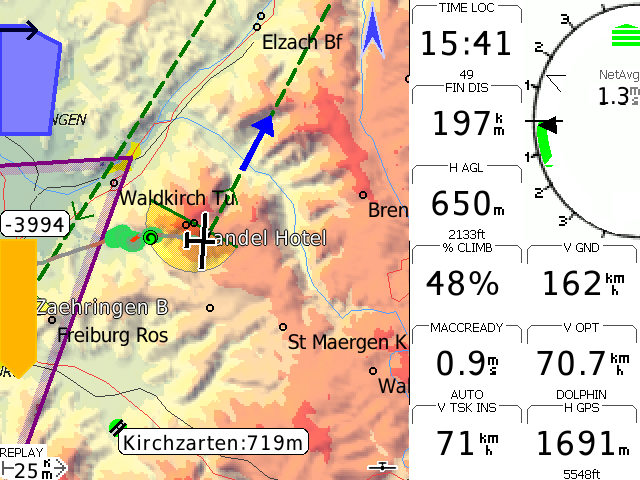
\includegraphics[angle=0,width=\linewidth,keepaspectratio='true']{figures/plain.png}
\caption{Typical XCSoar main screen layout}
\end{figure}

This chapter describes the fundamental user interface concepts used by 
XCSoar, and is intended as an overview. The \emph{main screen} covers much of 
the information needed during normal flight.  Typically, the main screen is 
composed of the moving map and infoboxes. For several reasons - not being the 
scope of an introduction - you have a choice of using several main screens 
in-flight, named \emph{screen pages}.

Screen pages are easily accessed by a horizontal swipe gesture just like 
turning pages of a book or button push, depending on the hardware you use. 
With screen pages you are enabled to compose several main screens to be used 
advantageously in different situations in-flight. Simply speaking, you are 
enabled to use appropriate information in different \emph{use cases}, to be 
accessed quite simply and fast. 

Whenever actual situations are worthy of grabbing the pilot's attention, an 
\emph{overlay} is put in front of the main screen. This happens especially 
when urgent reaction by the pilot is required as are the situation of a 
possible collision or an entering of a restricted airspace expected to happen
soon.

Evidently, menu buttons and menu screens are overlays too, and there are many 
more. As a result, the elements put on each other form a display stack with 
the main screen representing the base of it. More detailed descriptions are 
given in following chapters.



\section{Display elements}
\subsection*{Main screen and screen pages}
Every screen page out of XCSoar's screen pages' ensemble is composed of several 
parts:
\begin{description}
\item[Main area] The bulk of the screen typically is dedicated to the GPS moving 
map display. Various symbols relating to glide computer information are overlaid 
the map area. Icons and text may appear along the lower edge of the screen
to indicate status of connected devices, flight modes etc.
Following the development process of XCSoar there is an increasing number of 
items that may be chosen for display in the main area, which are gauges,
FLARM Radar, Thermal Assistant and Horizon.
\item[InfoBoxes] A grid of data values is displayed usually either along
the top and bottom of the screen (portrait display) or to the left and right of the
screen (landscape display).  These so-called InfoBoxes display data from the
GPS and other input devices as well as data calculated by XCSoar. Further, 
InfoBoxes can even display gauges and certain graphs.
\item[Bottom area] At the bottom of the screen, XCSoar is able to draw a cross-
section of terrain and airspaces in the direction of your heading.
\end{description}

\subsection*{Overlays}
\begin{description}
\item[Gauges]  Gauges provide instrumentation displays. All gauges are optional
and some may only have meaningful information displayed when XCSoar is
connected to a supported instrument.
A gauge overlay is either permanently drawn or is invoked by several 
conditions.  E.g.\ the thermal assistant is shown, when XCSoar enters circling
mode. The FLARM radar is invoked, whenever a probable collision is detected.
Permanently overlaid gauges are the final glide bar as well as the vario bar
amongst others.
\item[Button labels and menus] Hardware buttons on the device running XCSoar
can be used to bring up and navigate smaller on-screen menus that are
typically laid out such that menu items can be selected by pressing the
button adjacent to the item.  If the device has a touch screen, the menu
items can be selected by touching them.  These buttons are drawn in black
text on a grey background.
\item[Status messages] Text is displayed over the screen in status message
boxes.  This text is used to present detailed information to the pilot when
certain events occur.
\item[Dialogue windows] Larger dialogue windows, usually containing graphics and
buttons, are used to present detailed data to the pilot regarding waypoint
details, statistics and analysis etc.
\item[Main menu] The main menu is accessible by double tapping the map area or
InfoBoxes as well as through gesture. If the menu buttons are not pressed after
\gesturespec{du} a specified time, they disappear again so as to not obscure 
the map area.
\end{description}

\subsection*{Classic vario gauge}
As said above, gauges might be displayed in different ways, either as an 
infobox, overlay, or even in the main area. The traditional variometer gauge is 
different. This needle-style gauge is invoked permanently by choosing an infobox 
layout including the variometer on the right side of the other infoboxes. 

\section{Interaction}
There are several ways to interact with XCSoar:
\begin{itemize}
\item Touching certain map elements
\item Touching InfoBoxes and on-screen menu buttons
\item `Gesturing', by e.g.\ drawing a dash from the left to the right
  on the screen (see Section \ref{sec:gestures} below).
\item `Dragging' the screen (touching the screen and moving before releasing).
\item Pressing application buttons on the device.
\item Pressing the cursor keys on the device.
\item Pressing keys or switches on an instrument connected to XCSoar.
\end{itemize}
Depending on the particular hardware used with XCSoar, not all of these methods
of interaction are possible and there may be different numbers or assignments
of buttons.

For the PC version of XCSoar, clicking the mouse over an item is equivalent to
touching it.

\section{The main button menu}
The button menu is a set of buttons drawn on the screen and activated by touch
or hardware button presses.  Using buttons and the button menu is the primary
way the user interacts with XCSoar.

\subsection*{Interface basics}
The menu is organised into four different groups of functions, usually in
the form of a hierarchy.  The specific menu layout depends on the
hardware button configurations and platform, and may also be customised by the
user.

XCSoar can also accept input from external keyboards, game-pads, joysticks,
stick grip switches etc. A wide variety of functions can be assigned to these
inputs.
\sketch{figures/buttonmenu.png}

On the PC version, these mode buttons are activated by the
1, 2, 3 and 4 keys.  The 6, 7, 8, 9 and 0 keys correspond to the horizontal
strip of buttons.

If the user doesn't interact with the computer for some time, the
menu will close automatically.  This menu time-out is configurable.
The escape key on PC can also be used to close the current menu.

Menu buttons appear greyed out if the corresponding function is not available. 
For example, the ``Waypoint list'' function will appear grey if there are no waypoints loaded.

Several menu button labels have dynamic text based on context, in
order to make it clearer as to what happens when the button is
pressed.  The convention is used that a button's label describes what
will happen when the button is pressed.  For example, if the button
says \bmenug{MC Auto}, then pressing the button will turn on `Auto
MacCready', and the button label will then change to \bmenug{MC Manual}. 
In the menu list described below, generic labels are used.

\subsection*{Menu function groups}
This section describes the default layout of the menu system on all
platforms.  The functions performed by each button are explained more
fully in following chapters.

For the PC version, the keys 1, 2, 3 and 4 activate the 
corresponding menu.  The following menu item list has on the left side of most 
of the menu buttons links to the respective section. Follow them to get to all 
related details.

\section{Menu item overview}

\subsection*{Navigation menu}
\noindent\makebox[\textwidth]{%

\begin{tabularx}{1.44\textwidth}{c|ccccc}
\bmenus{Nav 1/2}
 & \bmenus{Task}
 & \bmenut{Previous}{Turnpoint}
 & \bmenut{Next}{Turnpoint}
 & \bmenut{Waypoint}{List}
 & \bmenus{Alternates} \\
see
 & \ref{cha:tasks}
 & \ref{sec:advanc-rest-tasks}
 & \ref{sec:advanc-rest-tasks}
 & \ref{sec:waypoint-selector-dialog}
 & \ref{sec:alternates} \\ \\
\bmenus{Nav 2/2}
 & \bmenut{Task}{Abort}
 & \bmenut{Mark}{Drop}
 & \bmenus{Target}
 & {}
 & {} \\
see
 & \ref{sec:taskabort}
 & \ref{sec:markers}
 & \ref{sec:waypointdetails}
\end{tabularx}}

You should not start using XCSoar without knowing about the `Alternates' feature. 
Any `Task' related item in the navigation menu is used for planned cross 
country flight and certainly the second step.

\subsection*{Display menu}
\noindent\makebox[\textwidth]{%

\begin{tabularx}{1.44\textwidth}{c|ccccc}
\bmenus{Display 1/2}
 & \bmenut{Zoom}{In}
 & \bmenut{Zoom}{Out}
 & \bmenut{Zoom}{Auto}
 & \bmenut{Info}{Cruise/...}
 & \bmenut{Pan}{On} \\
see
 & \ref{sec:zooming}
 & \ref{sec:zooming}
 & \ref{sec:zooming}
 & \ref{sec:screenpages}
 & \ref{sec:panning} \\ \\
\bmenus{Display 2/2}
 & \bmenut{Labels}{All/...}
 & \bmenut{Trail}{Full/...}
 & \bmenut{Terrain}{On/Off}
 & \bmenut{Topo.}{On/Off}
 & \bmenut{Airspace}{On/Off} \\
see
 & \ref{sec:maplabels}
 & \ref{sec:trail}
 & \ref{sec:terrain_topo}
 & \ref{sec:terrain_topo}
 & \ref{sec:terrain_topo}
\end{tabularx}}

Most of the display menu items are available on gestures, or special key 
short-cuts of your device. Once you are familiar with XCSoar you probably 
will use those menu items less frequently.

\subsection*{Configuration menu}
\noindent\makebox[\textwidth]{%

\begin{tabularx}{1.44\textwidth}{c|ccccc}
\bmenus{Config 1/3}
 & \bmenut{MacCready}{$+$}
 & \bmenut{MacCready}{$-$}
 & \bmenut{MacCready}{Auto}
 & \bmenus{Flight}
 & \bmenus{Wind} \\
see
 & \ref{sec:stf}
 & \ref{sec:stf}
 & \ref{sec:auto-maccready}
 & \ref{sec:flight-setup}
 & \ref{sec:wind-setup} \\ \\
\bmenus{Config 2/3} 
 & \bmenus{System}
 & \bmenus{Plane}
 & \bmenus{Devices}
 & \bmenut{File}{Manager}
 & \bmenus{Replay} \\
see
 & \ref{cha:configuration}
 & \ref{sec:glidepolar}
 & \ref{conf:comdevices}
 & {}
 & \ref{sec:logger-replay} \\ \\
\bmenus{Config 3/3} 
 & \bmenut{Logger}{Start}
 & \bmenus{Raw Logger}
 & \bmenus{Airspace}
 & \bmenus{Vega}
 & \bmenus{Profiles} \\
see
 & \ref{sec:logger}
 & \ref{sec:raw-logger}
 & \ref{sec:airspace-filter}
 & {}
 & {}
\end{tabularx}}

The configuration menu is typically part of the ground interaction with 
XCSoar. You are not expected to spend much time in-flight with tweaking 
the configuration, except you manually adjust wind or MacCready settings. 
The `Vega' item gives control over the  Vega intelligent variometer. This 
comprises a sub-menu.


\subsection*{Information menu}
\noindent\makebox[\textwidth]{%

\begin{tabularx}{1.44\textwidth}{c|ccccc}
\bmenus{Info 1/3}
 & \bmenut{FLARM}{Radar}
 & \bmenut{METAR}{TAF}
 & \bmenut{What's}{here?}
 & \bmenut{Check}{list}
 & \bmenus{Analysis} \\
see
 & \ref{sec:flarm-traffic}
 & \ref{sec:metar-taf}
 & {}
 & \ref{sec:checklist}
 & \ref{sec:analysis-climb} \\ \\
\bmenus{Info 2/3}
 & \bmenus{Status}
 & \bmenus{Weather}
 & \bmenut{Team}{Code}
 & \bmenut{FLARM}{Details}
 & \bmenut{Thermal}{Assistant} \\
see
 & \ref{sec:flight-status}
 & \ref{sec:weather-forecast}
 & \ref{sec:team-flying}
 & {}
 & \ref{sec:thermal-assistant} \\ \\
\bmenus{Info 3/3}
 & \bmenus{Credits}
 & \bmenus{Airspaces}
 & \bmenut{Message}{Repeat}
 & {}
 & {} \\
see
 & \ref{sec:credits}
 & 
 & 
 & 
 &
\end{tabularx}}

The information menu is always a good address, when not only a clue on 
how to set MacCready is requested, but rather more elaborate help on a 
larger scope tactical decision on your flight is requested. %TODO rewrite


\subsection*{The Vega variometer sub-menu of the configuration menu}
\noindent\makebox[\textwidth]{%

\begin{tabularx}{1.44\textwidth}{c|ccccc}
\bmenus{Vega 1}
 & \bmenut{Airframe}{Switches}
 & \bmenut{Setup}{Audio}
 & \bmenut{Manual}{Demo}
 & \bmenut{Setup}{Stall}
 & \bmenus{Accel} \\ \\
\bmenus{Vega 2}
 & \bmenut{ASI}{Zero}
 & \bmenut{Accel}{Zero}
 & \bmenus{Store}
 & \bmenut{Cruise}{Demo}
 & \bmenut{Climb}{Demo}
\end{tabularx}}

The functions in this sub-menu require the Vega intelligent variometer. 
The menu can only be accessed if `Vega' is selected as the connected device.

\subsection*{The pan mode sub-menu of the Display menu}

\noindent\makebox[\textwidth]{%

\begin{tabularx}{1.44\textwidth}{c|ccccc}
\bmenus{Pan}
 & \bmenut{Pan}{Off}
 & \bmenut{Zoom}{in}
 & \bmenut{Zoom}{out}
 & \bmenut{What's}{here?}
 & {} \\
see
 & \ref{sec:panning}
 & {}
 & {}
 & {}
 & {}
\end{tabularx}}

This sub-menu unfortunately overlays the full-screen map view of the pan mode.
 Its functions are quite evident, although the menu could be replaced by multi-touch
 technology or knobs. Besides the essential `exit pan mode'
 function the `What's here?' button offers brilliant access to the variety of
 information of the map.

\section{Default menu buttons}

When no menu is active, (so-called default mode), the horizontal row
of buttons perform the following functions (from left to right):

\begin{center}
\begin{tabular}{c c c c c c}
 PC: & 6 & 7 & 8 & 9 & 0 \\
& \bmenus{Flight} & \bmenut{Task}{Manager} & {} & \bmenus{Target} & \bmenut{Drop}{Mark} \\
\end{tabular}	
\end{center}

For all other versions in the default mode, the cursor keys perform
the following functions:
\begin{jspecs}
\item[Up key] Zoom in
\item[Down key] Zoom out
\item[Left key] Drop marker
\item[Right key] Toggle through normal/aux. InfoBoxes and full-screen
\item[Enter] Clear status message or suppress FLARM gauge if open and no warning
active
\end{jspecs}

\subsection*{Dynamic menu labels}
Certain menu items have dynamic labels to make it clearer what happens when the
menu item is selected.  Furthermore, items that are not available are greyed
out to indicate that selecting the menu item will not do anything.

The convention used for dynamic menu labels is for the labels to display the
action that will be performed once the menu item is selected. For example 
``Lights On'' will turn the lights on, and the menu will be updated to display
``Lights Off'', which would then if pressed turn the lights off. This
convention is used throughout XCSoar.

A selection of key dynamic menu items is presented below:
\begin{description}
\item[\bmenug{Next Turnpoint}]  
  Greyed out if the task is cleared, or if the active turnpoint is the
  finish. If the currently active turnpoint is the turnpoint prior to the 
  finish, this displays  ``Waypoint finish''.
\item[\bmenug{Previous Turnpoint}]  
  Greyed out if the task is cleared, or if the active turnpoint is the
  start and there are no multiple start points.  If there are multiple
  start points and the active turnpoint is the start, then this
  displays ``Cycle start'' to allow selection between the various
  start points.  If the active turnpoint is the first turnpoint after 
  the start, this displays ``Waypoint Start''.
\item[\bmenug{Labels All}]  
  This will turn on all labels available on the map. There are more options to 
  only show a reduced set of labels like ``Labels Task'', thus not cluttering the 
  screen too much.
\item[\bmenug{Target}]  
  Greyed out if the task is cleared or in task abort.
\end{description}


\section{InfoBoxes and screen pages}\label{sec:infoboxandpages}

The information displayed in the InfoBox fields can be selected from a
wide variety of options (listed in Chapter~\ref{cha:infobox}). These
fields can also be used to change for example the MacCready setting.

The specific number and layout of the InfoBox grid depends on the
screen orientation and the device's display size.  

For a 320x240 display
Pocket PC in portrait mode, there are four InfoBoxes above and four
InfoBoxes below the map display.  %TODO Update the example by considering something else than a Pocket PC
\sketch{figures/infoboxes.png}

A typical landscape layout has 9 InfoBoxes and the variometer gauge 
to the right of the map display. 
For larger displays up to 24 InfoBoxes may be displayed simultaneously.  

In order to gain clarity, the less infoboxes you choose to be displayed at once, 
the faster your reading will be. On the other hand, there are much too many 
InfoBox options a pilot would hardly reject. The number of possible InfoBox 
options already exceeded one hundred. That is why XCSoar offers two ways of 
managing even more options than Info\emph{boxes} count.

Depending on your flight's state, whether you are circling or cruising, you can 
let XCSoar change the content of each single InfoBox. As an example you might 
change the display of the actual average climb whilst circling to speed to fly 
when cruising. The switch is derived automatically by entering different 
\emph{flight modes} (see section \ref{sec:flightmodes}) executing a switch to 
another \emph{InfoBox set}.

Further, you can use screen pages to change InfoBox content manually, by 
assigning different Infobox sets to different pages (see following section).

To gain access to automatic switching InfoBoxes dependent on the flight mode, 
just let XCSoar run with its pre-configured setup from installation. To set up 
your personal version of Infoboxes go through the following procedure.
\begin{description}
\item[InfoBox geometry] Choose a basic Infobox geometry or layout.  This basic 
layout is maintained through any changes in-flight, affecting InfoBox content 
only.\config{interface-appearance}
\item[Choose Infobox set ``Auto''] Configure at least one screen page with the
choice of Infoboxes ``Auto''. As can be seen on the corresponding configuration
screen, there are more screen pages pre-defined. \config{screenpages}  These 
others are not needed to gain automatic switches by flight mode. They are for \emph{manually} turning through the screens defined by pages. 
\item[Define InfoBox sets] Put together the Infobox content you want to be 
displayed in three Infobox sets called ``Circling'', ``Cruise'', and ``FinalGlide''
respectively.\config{infobox_sets}
\end{description}  


\subsection*{Screen pages with different InfoBox sets}\label{sec:screenpages}

XCSoar allows the pilot to define various sets of InfoBoxes that are 
appropriate for ``normal'' states of flight.  Assuming circling,
cruising, or final glide as normal, XCSoar can switch corresponding Infobox 
sets automatically.

As you might imagine, there are countless cases, you wished you had another 
ensemble of information displayed at once.  For all of these more or less 
special situations you can define up to eight screen pages, reflecting the 
actual \emph{use case}. Just to draw a brief sketch of the possibilities 
introduced by the concept of screen pages, a few use cases are given. 
\label{par:use_case}
\begin{description}
\item[Familiarisation] Especially if you are a beginner, you might study 
computed values in-flight in advance of placing them in your ``normal'' InfoBox
ensemble - just to get familiar with the reading. To do so, create a new 
Infobox named ``test'' to be placed on an additional screen page brought in. In
any case you can go back to the screen you know by ``turning a page''
\item[Competition] If you are a pilot scratching the edge, you might want to 
gain benefit of XCSoar's numerous task- and competition-related computations. 
In order to get them related to the competition's phases, you might like the 
idea of defining two special use cases with pages for the phase before start, 
another one for whilst racing.  If you are in search of a specific value to
be displayed, give it a try in chapter \ref{cha:infobox} ``\nameref{cha:infobox}''.
There is a big chance you will find it.
\item[On the ground] As a manager on duty you might use a screen page, showing 
the ``FLARM Radar'' solely.  This might happen on a PC screen running XCSoar
being connected to a FLARM receiver.
\end{description}

Whatever you would like to display, take into account the use case and screen 
pages concept.

\gesturespec{left}
To go through the various screen pages, use gesture left/right (touch-screen), or via menu button in menu \bmenug{Display 1/2}, showing a dynamic label, changing accordingly to the screenpage's content to show up next:
\gesturespec{right}

\bmenut{Display}{1/2}\blink\bmenut{Info}{Circling}\blink\bmenut{Info}{Cruise}\blink\bmenut{Info}{FinalGlide}\blink\bmenut{Info}{...}


\subsection*{Modifying InfoBox content}

(This section applies only when a touch-screen or mouse is present.)

Some InfoBox values can be changed by the user by selecting (i.e.\ long-pressing) the
InfoBox with the touch-screen or mouse.  This brings up a small tabular dialogue:

\begin{description}
\item[\bmenuw{Edit}]  
  Allows the pilot to adjust the InfoBox setting (e.g.\ raise or lower the
  MacCready setting)

\item[\bmenuw{Setup}]
  Allows you to change the behaviour of the setting related to the InfoBox 
  (for example, changing from auto to manual MacCready mode); or 
  to change the InfoBox itself by pressing `\emph{Switch InfoBox}', then 
  choosing from a list of all available InfoBoxes.

\end{description}

Examples of InfoBoxes that can
be adjusted include MacCready setting, wind speed, and altitude (QNH).


\subsection*{Changing InfoBox sets}

An entire set of InfoBox can be composed by the `\emph{Setup System}' configuration 
dialogues on the `\emph{Look / InfoBox Modes}' and `\emph{Look / InfoBox Pages}' 
\ref{sec:infobox_sets} setup page. 
The dialogues give a wide variety to set up the look and feel of the XCSoar pages.  


\section{Status messages}

Status messages appear over the map area to present text for a short period of
time.  The message disappears after the time period has elapsed, and different
types of message have different periods. Additionally, status messages can be
made to disappear by acknowledging the message.  Acknowledgement is achieved by
either pressing the enter key, touching the status
message (on touch-screen devices) or clicking the screen (mouse enabled devices).

Additional user buttons may be assigned to a status message repeat function,
which brings up the last message again.
\sketch{figures/status-message.png}

Typical status messages include:
\begin{itemize}
\item Airspace queries
\item Airspace warnings
\item User interface events (e.g.\ changing display modes)
\item Glide computer events (e.g.\ take-off, turning waypoints)
\end{itemize}

Note that status messages do not appear while a dialogue is on screen, the
messages are buffered and displayed as soon as the dialogue is exited.


\section{Dialogue windows}\label{sec:dialog-windows}

XCSoar contains several dialogue windows that can be activated to bring up
additional information and are also used for more complex interactions with the
user, such as editing tasks and configuring settings.

Some dialogues simply display information, and require no user input. Other
dialogues contain data fields that can be modified or buttons that can be pressed.  

A cursor appears over the active button or data field. Pressing the up/down
arrow keys, the cursor will cycle
through the next or previous items. For list items and scrollable text, the
up/down arrow key moves the cursor up or down the list or text, and the
left/right arrow keys move the cursor up or down by one page in long lists.

For PDAs and PC versions, list items can be selected by touching the item (or
left-clicking with the mouse). Once a list item is selected, another touch
(left click) is equivalent to pressing the enter key.

Pressing the right/left arrow keys, the data field value under the
cursor can be modified. Pressing the enter key activates the button or
makes a selection from a list.

Dialogues are typically started from the button menu.  

Many of the dialogue windows have multiple pages of information and are controlled
in a consistent fashion. Press the \bmenuw{$<$} or \bmenuw{$>$} buttons to
select the next or previous page of the dialogue and the \bmenuw{Close} button 
to make the dialogue disappear.

The escape key on a PC can also be used to close dialogues.

The user must close the dialogue to return to the map view. When a dialogue
has been opened, the main button menu is disabled until the dialogue is closed.

In some dialogues, items that are not relevant or valid (such as AAT details when
flying a non-AAT task) are not displayed.

A summary of the major dialogues is presented below.
\begin{description}
\item[Flight setup] Used to modify the polar of the glider both before and
during flight, as well as to set the QNH pressure
\item[Wind] Used to modify or adjust the estimated wind magnitude and direction
\item[Waypoint details] Describes a waypoint in detail and has navigation
functions such as `GoTo' and `Insert in Task'
\item[Waypoint list] Used to select a waypoint from the waypoint database
\item[Task manager] Used to create, modify and view cross country tasks
\item[Analysis] Shows several pages of analysis and statistics about the flight
\item[Status] The status dialogues give summaries of the situation of the 
aircraft, system, task, start and times
\item[Configuration] Allows XCSoar and certain connected devices to be
configured
\item[Airspace filter] Controls enabling and disabling the display and warnings
of each airspace class
\item[Team code] Allows transfer of coordinates between FLARM team mates via a 
  code
\item[Devices]  Selection of various external devices (e.g.\ smart variometers,
  FLARM, etc.).
\item[Setup Plane]  Easy reconfiguration of the plane-dependent settings (e.g. 
  polar, competition ID, etc.) by choosing from a list of previously-created 
  plane profiles.
\end{description}

These dialogues are described in later chapters, with the exception of the
check-list, status and text entry dialogues, which are described below.


\subsection*{Check-list (dialogue example)}\label{sec:checklist}

The checklist dialogue can display several pages of user-defined free text.
Typically this is used for check-lists. It can be accessed via the menu.

\bmenut{Info}{1/3}\blink\bmenut{Check}{List}
\sketch{figures/checklist.png}

These check-lists may include: daily inspection, preflight,
out-landing, pre-landing, radio procedures, and aircraft rigging and
de-rigging instructions.  Since the check-lists may be long, the
up/down keys may be used to scroll through the text. Clicking the
\bmenuw{$<$} and \bmenuw{$>$} buttons selects the previous/next
checklist.


\subsection*{Text entry} \label{sec:textentry}

A text entry dialogue is used for entering text.  This is used for team
code entry, setting file names, waypoint editing, as well as entering
other configuration options, such as pilot name for the logger.

Two ways of entering text are provided. 

To enter text in `high score style', use the A+/A- buttons to adjust the 
\sketch{figures/textentry.png}
character under the cursor (underlined character). Clicking the \button{$<$} 
and \button{$>$} buttons move the cursor left/right.  

To enter text with the touch screen keyboard, press the letters of choice 
one after the other. In some dialogues (e.g.\ waypoint editing) only the next
\sketch{figures/textentry_keyboard.png}
letters matching to an entry in the database will be shown. For deleting the 
last letter use the \button{$<-$} button. The \button{Clear} button deletes all input.

Press \button{Ok} to validate, or \button{Cancel} to exit.


\section{Acoustic alert and sound feedback}

XCSoar generates sounds for different events, and can be configured to
have custom sounds for any event.  See Section~\ref{sec:status-file} for
details on customisation.

When XCSoar is connected to the Vega intelligent variometer, it sends
commands to Vega's speech system, to give verbal clues and warnings such as:
\begin{itemize}
\item Final glide through terrain
\item Approaching/passing a task waypoint
\item Airspace warnings
\end{itemize}

The XCSoar user interface also can connect sound feedback to the completion 
of any command like:
\begin{itemize}
\item Marker dropped
\end{itemize}


\section{Screen visuals}

Certain aspects of the look of items on the screen can be adjusted.
The most noticeable of these is whether to display InfoBoxes and
gauges in white on black (called inverse colours) or black on white.


\section{Help system}

A help system provides descriptive text for properties in most
dialogues.

\section{Interfacing with gestures}\label{sec:gestures}
As of version 6.0, XCSoar supports so-called `gestures'.

To use this feature hold down the finger on the 
touch-screen (or mouse button at the PC), draw a certain figure and release 
the touch-screen / mouse button. Depending on the figure that was drawn 
a certain function is activated. \sketch{figures/gesture1.png}

A specific gesture is defined by movements of the finger or the 
cursor in the four directions Up, Down, Left and Right. This means if 
you drag your finger down and afterwards to the right over the screen, 
\gesture{dr} the gesture ``DR'' is detected, which stands for ``Down-Right''.
It will bring up the waypoint list. The manual indicates an available 
gesture as shown here on the left side of the text body. Both the blue hand 
and pictogram of the movement are used to indicate a specific gesture, in this 
case move down then to the right. A list of generally available gestures is 
shown below. \gesturespec{dr}
\vspace{2em}

\subsection*{Most common or basic gestures:}
\begin{itemize}
\item[\raisebox{-1em}
{
\includegraphics[angle=0,width=0.1\linewidth,keepaspectratio='true']{figures/du.png}}] DU, denoting a check mark: Show main menu 
\item[\raisebox{-1em}
{
\includegraphics[angle=0,width=0.1\linewidth,keepaspectratio='true']{figures/up.png}}] U: Zoom in 
\item[\raisebox{-1em}
{
\includegraphics[angle=0,width=0.1\linewidth,keepaspectratio='true']{figures/down.png}}] D: Zoom out 
\item[\raisebox{-1em}
{
\includegraphics[angle=0,width=0.1\linewidth,keepaspectratio='true']{figures/left.png}}] L: Turn screen page pro-grade (Normal, Aux., Full-screen...) 
\item[\raisebox{-1em}
{
\includegraphics[angle=0,width=0.1\linewidth,keepaspectratio='true']{figures/right.png}}] R: Turn screen page retrograde (Normal, Full-screen...) 
\item[\raisebox{-1em}
{
\includegraphics[angle=0,width=0.1\linewidth,keepaspectratio='true']{figures/urdl.png}}] URDL, denoting a P: \textbf{P}an-mode. Might also be invoked by 
moving two fingers apart on the screen.
\end{itemize}
\vspace{2em}

\subsection*{More gestures available:}
\begin{itemize}
\item[\raisebox{-1em}
{
\includegraphics[angle=0,width=0.1\linewidth,keepaspectratio='true']{figures/dr.png}}] DR, denoting an L: Show the Select Waypoint dialogue similar to menu 
item Waypoint \textbf{L}ist
\item[\raisebox{-1em}
{
\includegraphics[angle=0,width=0.1\linewidth,keepaspectratio='true']{figures/rd.png}}] RD, denoting a T: opens the \textbf{T}ask Manager
\item[\raisebox{-1em}
{
\includegraphics[angle=0,width=0.1\linewidth,keepaspectratio='true']{figures/dl.png}}] DL: show the Alternates List
\item[\raisebox{-1em}
{
\includegraphics[angle=0,width=0.1\linewidth,keepaspectratio='true']{figures/ud.png}}] UD: enables Auto-Zoom
\end{itemize}
\vspace{2em}

\subsection*{Sophisticated dialogues:}
\begin{itemize}
\item[\raisebox{-1em}
{
\includegraphics[angle=0,width=0.1\linewidth,keepaspectratio='true']{figures/ldr.png}}] LDR, denoting a C: Show the \textbf{C}hecklist.

\item[\raisebox{-1em}
{
\includegraphics[angle=0,width=0.1\linewidth,keepaspectratio='true']{figures/urd.png}}] URD, denoting an A: Show the \textbf{A}nalysis dialogue.
\item[\raisebox{-1em}
{
\includegraphics[angle=0,width=0.1\linewidth,keepaspectratio='true']{figures/ldrdl.png}}] LDRDL, denoting an S: Open the \textbf{S}tatus dialogue
\end{itemize}
